%This work is licensed under the Creative Commons License Attribution 4.0 International (CC-BY 4.0)
%https://creativecommons.org/licenses/by/4.0/legalcode
\documentclass[rgb]{standalone}
\usepackage{tkz-euclide}
\definecolor{myorange}{hsb}{0.0833, 1, 0.8}
\definecolor{mygreen}{hsb}{0.3333, 1, 0.8}
\definecolor{myblue}{hsb}{0.5833, 1, 0.8}
\definecolor{mymagenta}{hsb}{0.8333, 1, 0.8}
\begin{document}
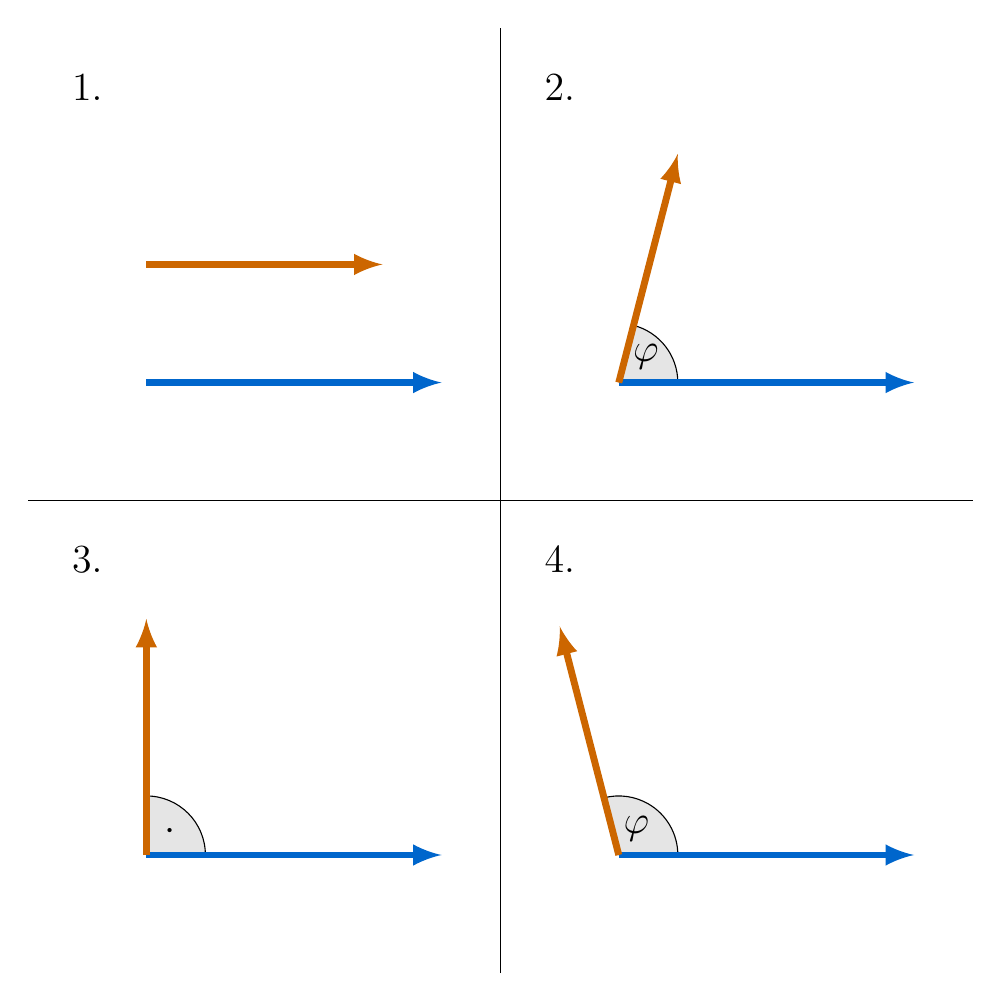
\begin{tikzpicture}[scale=1.5, font=\Large]
\draw[] (0,-4) -- (0,4);
\draw[] (-4,0) -- (4,0);
\draw[fill,fill opacity=0.1] (1,1) -- (1.5,1) arc (0:75.52:0.5);
\draw[fill,fill opacity=0.1] (-3,-3) -- (-2.5,-3) arc (0:90:0.5);
\draw[fill,fill opacity=0.1] (1,-3) -- (1.5,-3) arc (0:104.48:0.5);
\node[anchor=center] at (-2.8,-2.8){$\cdot$};
\draw[line width=2.5pt, myblue, -latex] (-3,1) -- (-0.5,1);
\draw[line width=2.5pt, myorange, -latex] (-3,2) -- (-1,2);
\draw[line width=2.5pt, myblue, -latex] (1,1) -- (3.5,1);
\draw[line width=2.5pt, myorange, -latex] (1,1) -- (1.5,{1+sqrt(15)/2});
\draw[line width=2.5pt, myblue, -latex] (-3,-3) -- (-0.5,-3);
\draw[line width=2.5pt, myorange, -latex] (-3,-3) -- (-3,-1);
\draw[line width=2.5pt, myblue, -latex] (1,-3) -- (3.5,-3);
\draw[line width=2.5pt, myorange, -latex] (1,-3) -- (0.5,{-3+sqrt(15)/2});
\node[above=0.5mm] at (1.23,1){$\varphi$};
\node[above=0.5mm] at (1.15,-3){$\varphi$};
\node[anchor=center] at (-3.5,3.5){$1.$};
\node[anchor=center] at (0.5,3.5){$2.$};
\node[anchor=center] at (-3.5,-0.5){$3.$};
\node[anchor=center] at (0.5,-0.5){$4.$};
\end{tikzpicture}
\end{document}